\chapter*{Open Composition}
\phantomsection

\addcontentsline{toc}{chapter}{Open Composition}

 %« 
 << \textit{I musicisti futuristi deveno allargare ed arrichirre sempre pi\`{u} il campo dei suoni.}  >>\footnote{Luigi Russolo, \textit{L'Arte dei rumori}, 1913, Conclusioni 1.} 
 %»

\section*{Prol\'{e}gom\`{e}nes}
\phantomsection

\addcontentsline{toc}{section}{Prol\'{e}gom\`{e}nes}
\thispagestyle{empty}

<< \textit{Everything we do is music.} >>\footnote{John Cage in: Richard Kostelanetz, \textit{Conversing with Cage}, 2003, p. 74.}

\bigskip

%De la musique tonale au contrepoint rigoureux jusqu'au free jazz, la composition offre sinon une infinit\'{e}, du moins une pl\'{e}thore de modalit\'{e}s. Il s'agit bien sûr de modalit\'{e}s compositionnelles, qui souvent sont convenu en tant que st\'{e}r\'{e}otype, contenu en tant qu'arch\'{e}type ou en devenir en tant que proptotype.

\renewcommand{\labelenumii}{\arabic{enumi}.\arabic{enumii}.}
%\renewcommand{\labelenumiii}{\arabic{enumi}.\arabic{enumii}.\arabic{enumiii}}
%\renewcommand{\labelenumiv}{\arabic{enumi}.\arabic{enumii}.\arabic{enumiii}.\arabic{enumiv}}

 \noindent Du concept ... 
 \begin{enumerate}[itemsep=0pt]
 \item Historique 
 	\begin{enumerate}[itemsep=0pt,topsep=1pt]
 		\item 1913 << \textit{L'Arte dei rumori} >> [ Luigi Russolo ] 
 		\item 1916 << \textsl{Ready-made} >> [ Marcel Duchamp ] 
 		\item 1939 Musiques << exp\'{e}rimentales >> [ John Cage ] 
 		\item 1967 << Le temps de le prendre >> [ Jean-Yves Bosseur ] 
 	\end{enumerate}
 \item Formalisation d'id\'{e}es directrices 
 	\begin{enumerate}[itemsep=0pt,topsep=1pt]
		\item musicales 
 		\item formelles 
 		\item structurelles 
 		\item interrelationnelles 
 		\item interactionnelles 
  	\end{enumerate}
 \item Intelligibilit\'{e} du discours musicales en termes 
  	\begin{enumerate}[itemsep=0pt,topsep=1pt]
 		\item intellectuelles 	
 		\item exp\'{e}rientielles
  	\end{enumerate}
 \end{enumerate}
\noindent ... \`{a} la \textit{praxis} 
 \begin{enumerate}[label=\alph*.,itemsep=0pt]
\item \textit{In vivo} et \textit{in situ}
\item Accessibilit\'{e} \`{a} tout un chacun 
\item Partage des savoirs et des connaissances.
 \end{enumerate}


\bigskip

\noindent << Comment comprendre la musique conceptuelle? Le processus de s\'{e}lection d'un \textsl{ready-made} nous donne des \'{e}l\'{e}ments de r\'{e}ponse. Dans L'\OE{}uvre de l'art, G\'{e}rard Genette explique, \`{a} propos de cet objet industriel \'{e}lev\'{e} au rang d'\oe{}uvre d'art par un artiste d\`{e}s 1913\footnote{\textit{i.e.} Marcel Duchamp.}, que la repr\'{e}sentation intellectuelle v\'{e}hicul\'{e}e par le ready-made est consid\'{e}rable: ce qui importe n'est `ni l'objet propos\'{e} en lui-m\^{e}me, ni l'acte de proposition en lui-m\^{e}me, mais l'id\'{e}e de cet acte'. >> \citep[\S11]{stso}%\footnote{Sophie St\'{e}vance, \textit{Les op\'{e}rations musicales mentales de Duchamp. De la} << \textit{musique en} \hbox{\textit{creux} >>}, 2009, §11.}

\bigskip

\textsl{From tonal music with its rigorous counterpoint to free jazz, the composition offers, if not an infinity, at least a plethora of modalities. We are talking about compositional modalities, which often are agreed upon stereotypes, identified as archetypes, or emerging as prototypal.}
\bigskip

\noindent << Noter, ce n'est plus n\'{e}cessairement indiquer une hauteur de son, un rythme ... noter, c'est aussi inventer une \'{e}criture. >> \citep[p.~133]{bos}%\footnote{Jean-Yves Bosseur, \textit{Du son au signe. Histoire de la notation musicale}, 2005, p. 133.}

\bigskip

\section*{\textsl{Diwar Les Coet}}
\phantomsection

\addcontentsline{toc}{section}{\textsl{Diwar Les Coet}}

\bigskip

\begin{description}
\item[Concept] \hfill 
\begin{itemize}
\item[--] Un espace \`{a} occuper
\item[--] Un ensemble de musiciens, en petits groupes, formations, ou bien solistes  
\item[--] Des partitions
\item[--] Un tempo commun 
\item[--] Une performance 
\end{itemize}
\bigskip
\item[Context] \hfill 
\begin{itemize}
\item[] Initialement \'{e}crit pour le Refuge des loups de Coat Fur dans le cadre d'un `mini festival' sur une ou deux journ\'{e}es, le projet rest\^{a}t en l'\'{e}tat. \\ $\rightarrow$ \href{http://refugedesloups.org}{\texttt{\small http://refugedesloups.org}}
\end{itemize}
\bigskip
\item[Notes] \hfill 
\begin{itemize}
\item[--] L'\textit{espace \`{a} occuper} doit \^{e}tre suffisamment grand pour discerner les diff\'{e}rents intervenants comme autant de `\textit{stages}', mais pas trop de fa\c{c}on \`{a} percevoir la plupart d'entre eux dans les espaces `neutres'.
\item[--] Les \textit{partitions} doivent se construire \`{a} partir ou s'inspirer des sch\'{e}mas harmoniques et rythmiques propos\'{e}s en annexe page \pageref{dlcscore}.
\item[--] Le \textit{tempo commun} consiste \`{a} une synchronisation formelle pour l'en- semble des participants. Cela peut se faire avec l'application INScore par exemple, d\'{e}crit en annexe page \pageref{inscore}.
\item[--] La \textit{perfomance} requiert une concertation apriori entre les participants afin de r\'{e}aliser un parcours formel (enchainement, superposition, tempo, ...).
\end{itemize}

\begin{enumerate}

\item Les possibles dissonances comme autant de couleurs harmoniques -- notamment intergroupe mais pas que -- ne doit pas rebuter les participants. Il convient de rester concentrer sur sa partition au tempo donn\'{e}.

\myuline{Le concept lui-m\^{e}me repose sur les superpositions intergroupes.}

\item Il est \`{a} pr\'{e}ciser que ce type d'interpr\'{e}tation ne mobilise pas tous le monde tous le temps (sauf pour les \textit{tutti}). Aussi, une `mise en sc\`{e}ne' ou une `th\'{e}\^{a}tralisation' de la performance -- pouvant reposer sur un texte et par cons\'{e}quent sc\'{e}narisable -- est \`{a} prendre en compte, afin que chacun se rep\`{e}re dans le temps sans \^{e}tre clou\'{e} \`{a} son instrument ou \`{a} sa place durant toute la performance.

\item Pour finir, la performance doit \^{e}tre interpr\'{e}t\'{e}e sans aucune sonorisation -- sauf effet acoustique irr\'{e}alisable autrement ou pour les instruments d\'{e}finitivement \'{e}lectriques et ce, dans le respect de l'\'{e}quilibre sonore de l'ensemble.

\item L'effectif minimal envisageable est de 9 personnes -- 3 voix (basse, baryton et t\'{e}nor), un djemb\'{e}, un dumdum et 4 guitares.
 \end{enumerate}

% L'effectif maximal est quant \`{a} lui illimit\'{e}.

%\begin{itemize}
%\setlength\itemsep{1em}
%\item[] ...
%\end{itemize}
%\bigskip
%\item[Source] \hfill 
%\begin{itemize}
%\item[] ...
%\end{itemize}
\end{description}

\bigskip

\begin{center}\rule{0.5\linewidth}{0.5pt}\end{center}

\bigskip

\section*{Nord}
\phantomsection

\addcontentsline{toc}{section}{Nord}

\bigskip

\begin{description}
\item[Concept] \hfill 
\begin{itemize}
\item[--] One Spirit
\item[--] Two chords
\item[--] Three movements
\item[--] A workshop
\item[--] The performance
\item[--] An \textit{egregore}
\end{itemize}
\bigskip
\item[Context] \hfill 
\begin{itemize}
\item[] The quest for the pole.
\end{itemize}
\bigskip
\item[Workshop] \hfill 
\begin{itemize}
\item[--] One movement will be a collective composition with graphical score involving the creativity of every participant, according to the constituent elements or the spirit of this Open Composition.  
\item[--] Another one movement, only based on rhythm, consist to follow a diagram as the graphical conductor score. 
 \begin{figure}[H]
\begin{center}
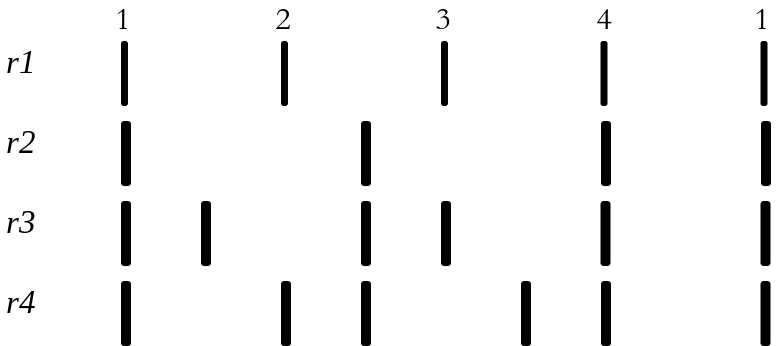
\includegraphics[scale=0.3]{img/nrtm}
\end{center}
\end{figure}
This diagram (see annex INScore page ... for further detail) is repeated as many time as needed in order to start very slow, then increasing the pulsation gradually until very fast. If some participant drop out during the \textit{accelerando}, the leader(s) will take over dynamically (\textit{i.e. crescendo forte fortissimo} then \textit{subito} silent or \textit{decrescendo perdendosi}).
\item[--] Another one movement, will be based on the chord diagrams on annex page \pageref{oco2}. Each musician or group leader are invited to create their own variation.
\item[--] An Interlude as a duet, for one guitar according to the score in annex page \pageref{interlude} and ideally one wind instrument.
\end{itemize}
\bigskip
\item[Notes] \hfill 

To introduce the musical event itself, there are some general recommendations to be followed.
\begin{enumerate}
\item The performance should be done as far as possible outside and without any amplification, except for some special effect. Also, the performers should be all around and even among the audience in order to occupy all space available.
\item There is no limit for the duration of each part of the performance, and no limitation for the number of performers involved.
\item Each soloist is free to act at any moment during the performance.
\item The order of the movements has to be defined by the participants, including the Interlude.
 \end{enumerate}
\end{description}

\bigskip
\begin{center}\rule{0.5\linewidth}{0.5pt}\end{center}
\bigskip

\section*{\textsl{Kj{\o}lhiea}}
\phantomsection

\addcontentsline{toc}{section}{\textsl{Kj{\o}lhiea}}

\bigskip

\begin{description}
\item[Concept] \hfill 
\begin{itemize}
\item[--] A prayer
\item[--] Patterns
\item[--] Performances
\end{itemize}
\bigskip
\item[Context] \hfill 
\begin{itemize}
\item[] ... \textit{et le vent souffle au sommet de la montagne.} 

\textit{La nuit, par rafales} ...
\item[]
\item[] Electronic versions in quadraphony:
\item \texttt{K540} version 1 (see description page \pageref{k540v1}) -- interpreted the 29th of January, 2018 -- \textit{Kulturhuset Hausmania} -- Oslo.
\item \texttt{K540} version 2 (see description page \pageref{k540v2}) -- interpreted the 7th and the 8th of June, 2019 -- \textit{UddeboFestidalen} -- Sweden.

$\rightarrow$ \href{http://uddebo.uddetopia.com/uppleva-gora/uddebofestidalen}{\texttt{\small http://uddebo.uddetopia.com/uppleva-gora/uddebofestidalen}}

\item \texttt{K540} version 3 (see description page \pageref{k540v3}) -- interpreted the 27th and the 28th of July, 2019 -- \textit{Trans' Festival}  -- Norway.
\end{itemize}
\item[Source] \hfill 
\begin{itemize}
\item[] \textit{Inspir\'{e} par un chant dont l'origine et la source se perd dans ma m\'{e}moire, dont les mots eux-m\^{e}me m'\'{e}chappent, comme une pri\`{e}re herm\'{e}tique, l'harmonie reste.}
\end{itemize}
\bigskip
\bigskip
\item[Notes] \hfill 
\begin{itemize}
\item[]  The initial idea of \textsl{Kj{\o}lhiea} was to confront a guitar quartet (see appendix page \pageref{kjccqg}, section \textsl{for 4 guitars}) -- while allowing them a space of freedom, as much in terms of improvisation as in terms of a free interpretation, which could be based on chord diagrams for instance (see appendix page \pageref{kjcccc}, section \textsl{chord diagrams}) -- with an algorithmic composition for quadraphonic installation. The latter has been performed on several occasions as a solo piece under the title of K540 (see \textsl{context} point above).
%L'id\'{e}e initiale de \textsl{Kj{\o}lhiea} \'{e}tait de confronter un quatuor de guitares, jouant sur la partition du m\^{e}me nom (voir annexe \ref{kj} page \pageref{kj}), tout en leur laissant un espace le libert\'{e}, autant en termes d'improvisation que sur une interpr\'{e}tation libre, pouvant reposer par exemple sur le diagramme d'accords en annexe page \pageref{kjcc}, avec une composition pour dispositif \'{e}lectronique en quadriphonie. Laquel a \'{e}t\'{e} r\'{e}alis\'{e} en `solo' \`{a} plusieurs reprises sous le titre \texttt{K540} (voir § \textsl{context} ci-dessus).
\end{itemize}

%\bigskip
%\item[Source] \hfill 
%\begin{itemize}
%\item[] ...
%\end{itemize}
\end{description}


\bigskip

\begin{center}\rule{0.5\linewidth}{0.5pt}\end{center}

\bigskip

